\documentclass{sdqbeamer}

\titleimage{banner_2020_kit}
\groupname{Modelling for Continuous Software Engineering}
\grouplogo{}

\title{Generierung von UML-Diagrammen aus PCM-Modellen}
\subtitle{Praktikum: Werkzeuge für agile Modellierung WS 2021/22}
\author{Sonya Voneva}

\date[21.03.22]{21. März 2022}

\usepackage{listings}
\begin{document}
\KITtitleframe

\begin{frame}{Inhaltsverzeichnis}
\tableofcontents
\end{frame}

\section{Motivation}
\begin{frame}{Motivation}
\begin{greenblock}{Visualisierung wichtig}
besseres Verständnis, Fehlererkennung  \texttt{}
\end{greenblock}
\pause
\begin{greenblock}{Schnelle, parallele Übersicht}
neben dem Baum-/Texteditor  \texttt{}
\end{greenblock}
\pause
\begin{greenblock}{Vorherige Darstellung}
zu komplex, skaliert nicht gut  \texttt{}
\end{greenblock}
\end{frame}

\begin{frame}
    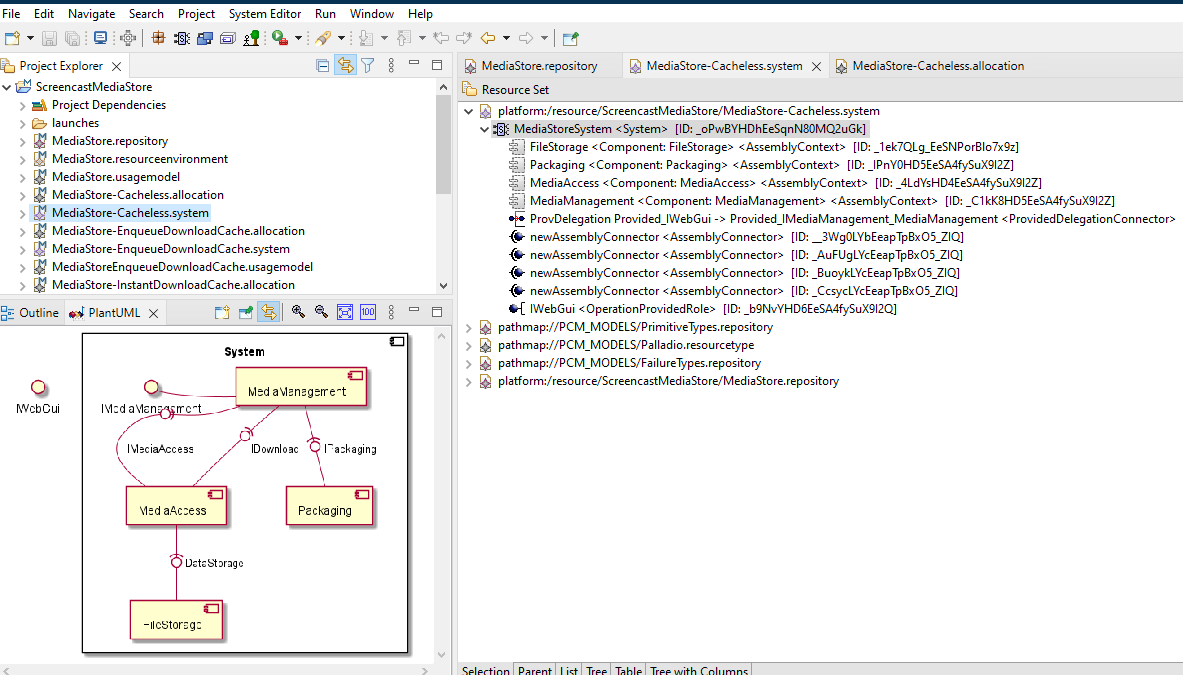
\includegraphics[width=\textwidth]{plantuml+repo.png}
\end{frame}

\section{Grundlagen}
\subsection{Palladio}
\begin{frame}{Palladio Framework}
\begin{columns}
\column{.3\textwidth}
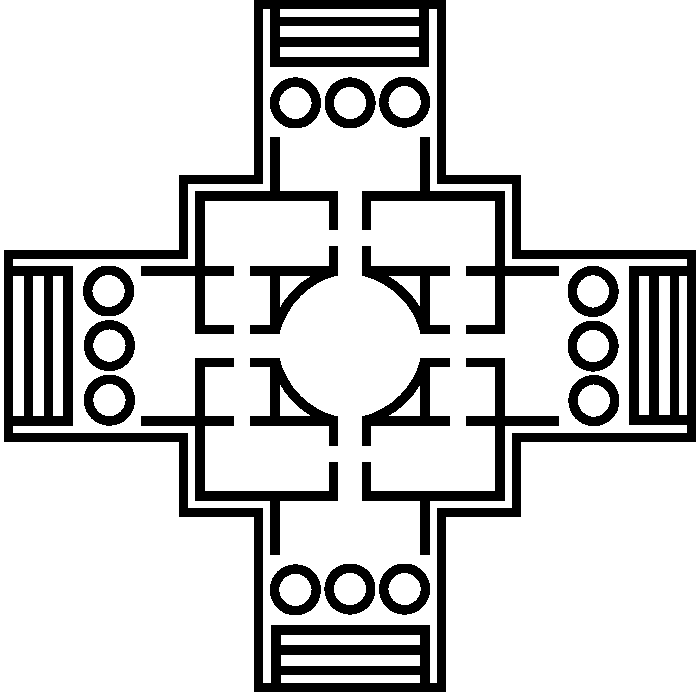
\includegraphics[width=\textwidth]{palladio.pdf}
\column{.7\textwidth}
\begin{itemize}
\item Domain-specific Modeling Language
\item Aussagen über die Qualität-Eigenschaften von Software
\item Tools: graphische Editoren, verschiedene Modelltypen, Simulationsengine
\end{itemize}
\end{columns}
\end{frame}
\begin{frame}
\centering
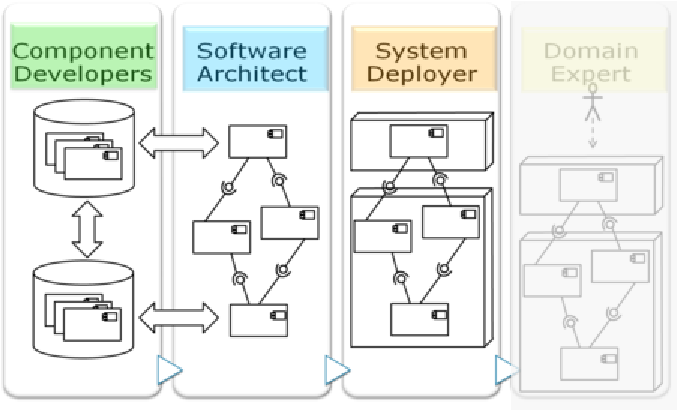
\includegraphics[width=.8\textwidth]{palladio_sichten.drawio.pdf}
\end{frame}

\subsection{PlantUML}
\begin{frame}{PlantUML}
\begin{columns}
\column{.7\textwidth}
\begin{itemize}
\item Erstellen von UML Diagrammen durch textuelle Notation
\item Online Editor, Integration in Eclipse
\item Beispiel: 
\begin{figure}[t]
    \centering
    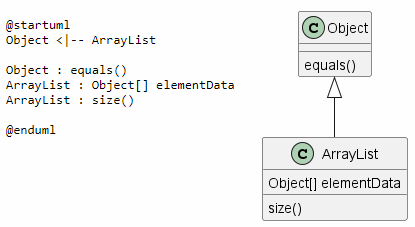
\includegraphics[width=.75\textwidth]{plantuml_beispiel.png}
\end{figure}
\end{itemize}

\column{.3\textwidth}
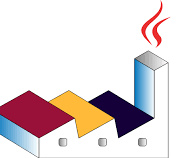
\includegraphics[width=.6\textwidth]{plantuml.jpg}
\end{columns}
\end{frame}

\subsection{Eclipse Plugin}
\begin{frame}{Eclipse Plugin}
\begin{columns}
\column{.7\textwidth}
    \begin{itemize}
        \item PlantUML - in Plugins aufgeteilt
        \item Funktionalität von Eclipse Plugin wiederverwenden
        \item Einfache Erweiterung
    \end{itemize}
    
\column{.2\textwidth}
    
\includegraphics[width=\textwidth]{eclipselogo.jpg}
\end{columns}
\end{frame}

\section{Transformationen}
\subsection{Ansatz}
\begin{frame}{Ansatz}
\begin{enumerate}
\item Eigenes Bundle erstellen
\item Eigene Klasse für jeden Diagrammtyp
\item Durch die Palladio Modellelemente iterieren -> in die textuelle PlantUML Notation "übersetzen"
\item Hyperlinks (z.B zu Repository) hinzufügen
\end{enumerate}
\end{frame}

\subsection{Architektur}
\begin{frame}{Architektur}
    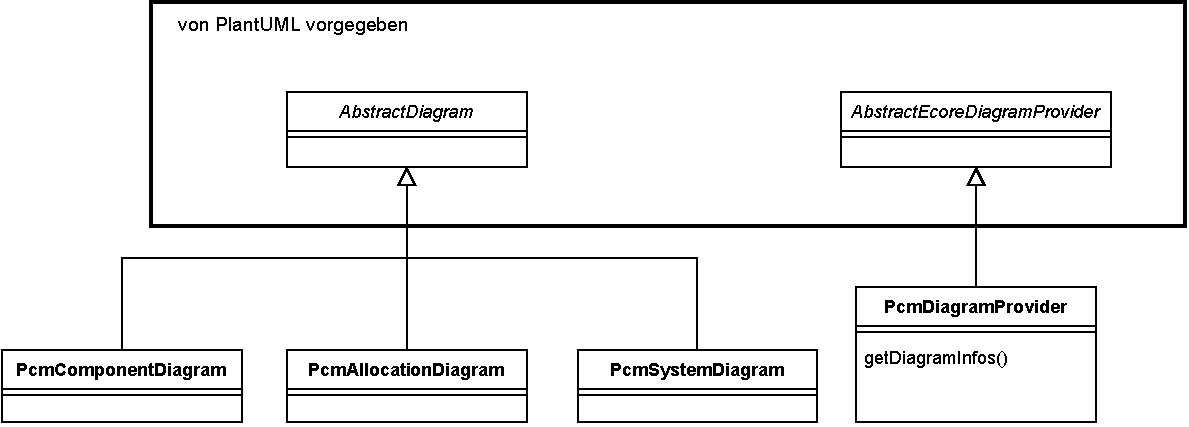
\includegraphics[width=\textwidth]{klassendiagramm.drawio.pdf}
\end{frame}

\begin{frame}[fragile]{PlantUML Notation}
\begin{columns}
\column{.5\textwidth}
\begin{lstlisting}[basicstyle=\small]
@startuml
skinparam fixCircleLabelOverlapping true
() IWebGui
component System {
    IWebGui - IMediaManagement
    IMediaManagement - [MediaManagement]
    [MediaManagement] -(0- [MediaAccess] : IMediaAccess
    [MediaManagement] -(0- [MediaAccess] : IDownload
    [MediaAccess] -(0- [FileStorage] : IDataStorage
    [MediaManagement] -(0- [Packaging] : IPackaging
    [FileStorage] 
    [Packaging]
    [MediaAccess] 
    [MediaManagement]
}
@enduml
\end{lstlisting}

\column{.5\textwidth}
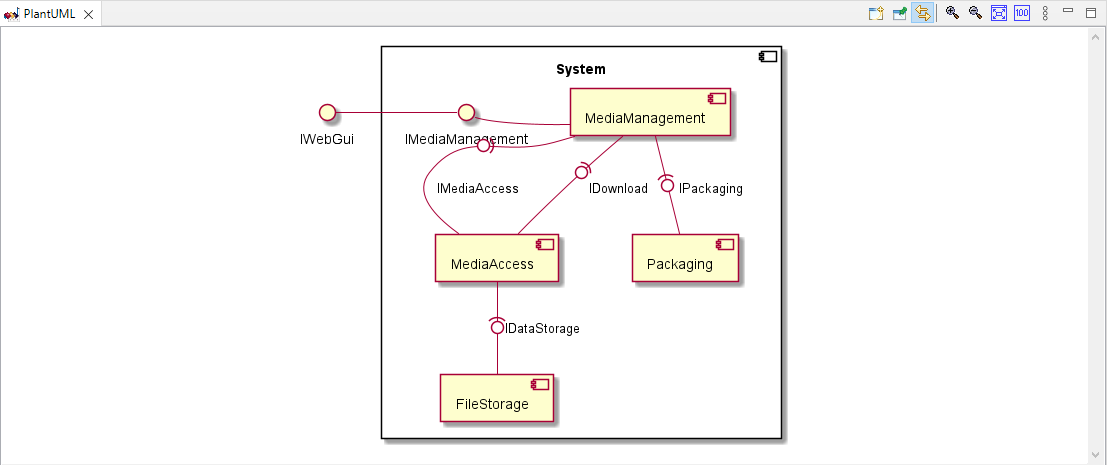
\includegraphics[width=\textwidth,height=.8\textheight]{system.png}
\end{columns}
\end{frame}

\subsection{PlantUML Diagramme}
\begin{frame}{Repository-Diagramm}
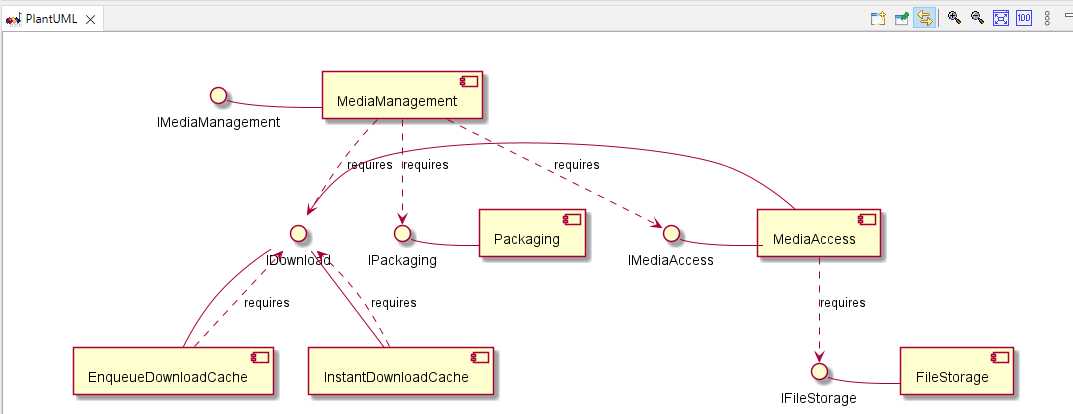
\includegraphics[width=\textwidth]{repository.png}
\end{frame}
\begin{frame}{Systemdiagramm}
\centering
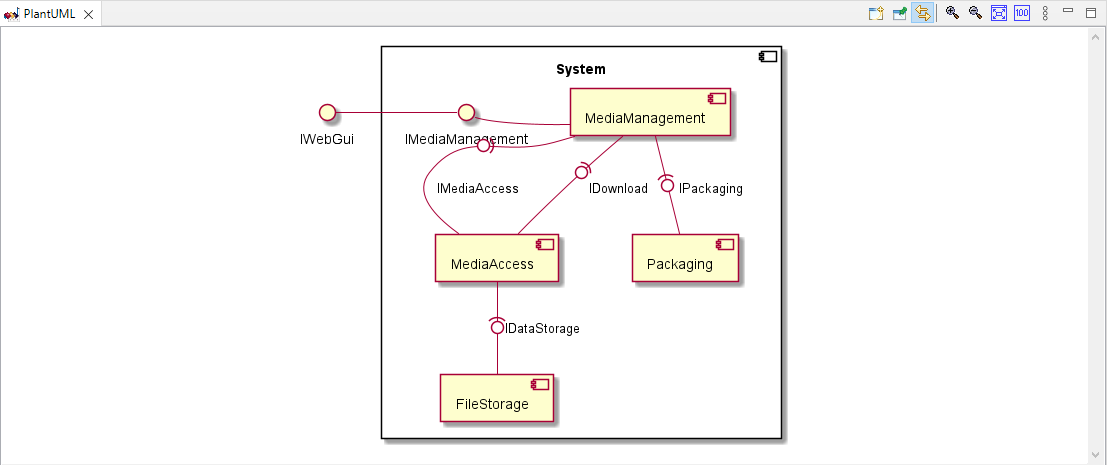
\includegraphics[height=.8\textheight]{system.png}
\end{frame}
\begin{frame}{Allocation-Diagramm}
\centering
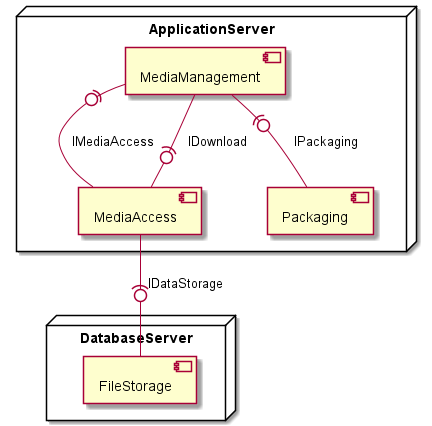
\includegraphics[height=.8\textheight]{allocation.png}
\end{frame}

\begin{frame}{Continuous Integration}
\begin{itemize}
    \item Bundle ist Teil von einer Continuous Integration Pipeline
    \item Quelltext + Dokumentation automatisch gebaut, verifiziert, deployed
    \item Bundle theoretisch über die Updateseite installierbar
\end{itemize}
\centering
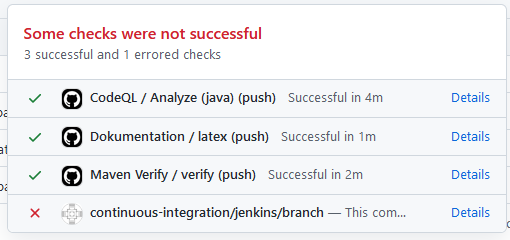
\includegraphics[width=.6\textwidth,height=.5\textheight]{github.png}

\end{frame}

\section{Einschränkungen}
\begin{frame}{Einschränkungen}
\begin{redblock}{Diagramme nicht interaktiv}
nicht direkt graphisch editierbar \texttt{}
\end{redblock}
\pause
\begin{redblock}{PlantUML Algorithmen}
Auto-Layout, Rendering, überlappende Labels \texttt{}
\end{redblock}
\end{frame}

\section{Zusammenfassung}
\begin{frame}{Zusammenfassung}
    \begin{itemize}
        \item PlantUML um ein neues Bundle erweitert
        \item Elemente von Repository-, System- und Allocation-Modell abgebildet
        \item Teil vom Continuous Integration Ansatz 
    \end{itemize}
\end{frame}

\end{document}